%----------------------------------------------------------------------------------------
%    PACKAGES AND THEMES
%----------------------------------------------------------------------------------------

\documentclass[aspectratio=169,xcolor=dvipsnames]{beamer}
\usetheme{SimplePlus}

\usepackage{hyperref}
\usepackage{graphicx} % Allows including images
\usepackage{caption}
\usepackage{booktabs} % Allows the use of \toprule, \midrule and \bottomrule in tables
\usepackage{enumitem}
\usepackage{float}
\usepackage{wrapfig}
\usepackage{natbib}
\usepackage{xcolor}
\usepackage{stmaryrd}
\usepackage{soul}

\sethlcolor{yellow}

\setbeamercolor{block title alerted}{bg=yellow!35, fg=black}
\setbeamercolor{block body alerted}{bg=yellow!12, fg=black}


%----------------------------------------------------------------------------------------
%    TITLE PAGE
%----------------------------------------------------------------------------------------

\title{Stochastic Model of Local Fluctuating Magnetic Fields in Pulsed NMR}
\subtitle{}

\author{Luca Roncoroni Seda}

\institute
{
    University of Southern California, Department of Physics \& Astronomy\\
    PHYS 493
}
\date{April 27, 2026} % Date, can be changed to a custom date

%----------------------------------------------------------------------------------------
%    PRESENTATION SLIDES
%----------------------------------------------------------------------------------------

\begin{document}

\begin{frame}
    % Print the title page as the first slide
    \titlepage
\end{frame}

%------------------------------------------------

\begin{frame}{Introduction to Pulsed NMR}
    \begin{minipage}[t]{0.45\textwidth}
        \begin{figure}
            \centering
            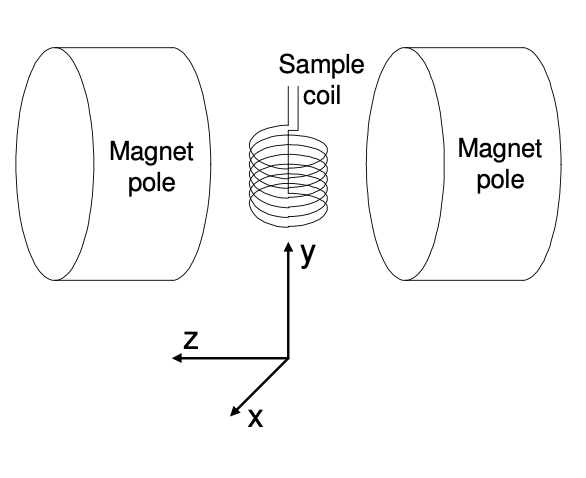
\includegraphics[width=\linewidth]{figures/coil_magnet.png}
            \captionof{figure}{Magnet and coil set-up [TeachSpin Pulsed/CW NMR Manual]}
        \end{figure}
    \end{minipage}
    \hfill
    \begin{minipage}[t]{0.5\textwidth}
        \begin{block}{Physical picture}
            \begin{itemize}
                \item[$\bullet$] Place a sample in a strong magnetic field and briefly hit it with a radiofrequency (RF) pulse.
                \item[$\bullet$] After the pulse, the sample emits a decaying oscillatory signal.
            \end{itemize}
        \end{block}
        \vspace{10pt}
        \textbf{Question:}
        \begin{itemize}
            \item What causes the decay, and what information about the system does it incode?
        \end{itemize}
    \end{minipage}
\end{frame}

%------------------------------------------------

\begin{frame}{Spin precession, magnetization, and RF pulses}
    \begin{minipage}{0.5\textwidth}
        Spins behave like tiny magnets
        \begin{itemize}
            \item[$\bullet$] In a magnetic field
                \begin{equation*}
                    \omega_0 = \gamma B_0
                \end{equation*}
            \item[$\bullet$] Net magnetization $M_0$ aligns along $z$ in thermal equilibrium
        \end{itemize}
        RF pulse creates a measurable signal
        \begin{itemize}
            \item[$\bullet$] $M_0$ is tipped onto $xy$-plane
            \item[$\bullet$] Spins precess coherently $\rightarrow$ oscillating signal
        \end{itemize}
    \end{minipage}
    \hfill
    \begin{minipage}{0.45\textwidth}
        \begin{figure}
            \centering
            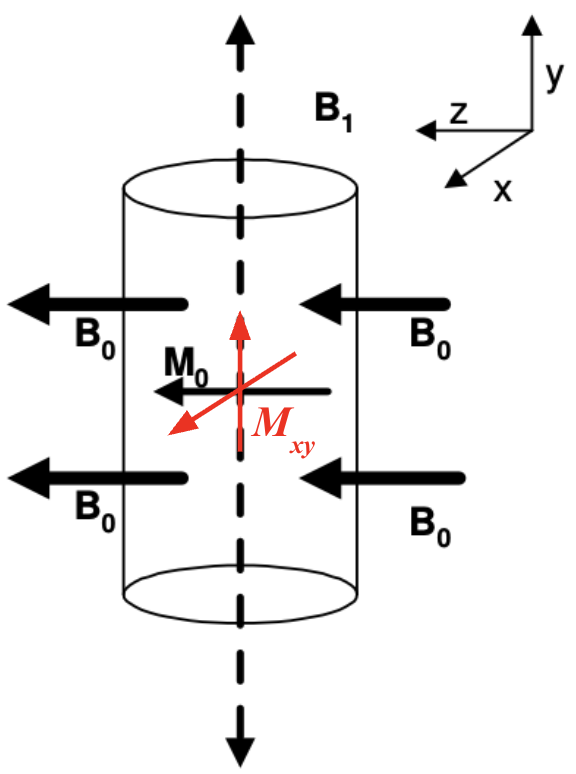
\includegraphics[width=0.7\linewidth]{figures/sample.png}
        \end{figure}
    \end{minipage}
\end{frame}

%------------------------------------------------

\begin{frame}{Decay of the transverse magnetization}
    The transverse magnetization will decay exponentially:
    \begin{equation*}
        M_{xy} (t) = M_0 e^{-t/T_2}
    \end{equation*}
    \begin{block}{$T_2$ -- Spin-spin relaxation time}
        The timescale for loss of phase coherence...
    \end{block}
    \vspace{15pt}
    \begin{minipage}{0.45\textwidth}
        \textbf{Interpretation:}
        \begin{itemize}
            \item Decay = loss of phase coherence among spins
        \end{itemize}
    \end{minipage}
    \hfill
    \begin{minipage}{0.5\textwidth}
        \textbf{Question:} 
        \begin{itemize}
            \item What causes this loss of coherence, and how can we model it?
        \end{itemize}
    \end{minipage}
\end{frame}

%------------------------------------------------

\begin{frame}{Phase decoherence}
    The signal could decay via two mechanisms:
    \begin{itemize}
        \item \textbf{Field inhomogeneity} -- the static field varies across the sample (\textit{reversible})
        \item \textbf{Time-dependent fluctuations} -- fields change in time due to molecular dynamics (\textit{irreversible})
    \end{itemize}
    Both result in a \textit{distribution} of precession frequencies $\rightarrow$ loss of phase coherence.
\end{frame}

%------------------------------------------------

\begin{frame}{Spin echo}
    We can indeed reverse the effect of field inhomogeneity
    \begin{figure}
        \centering
        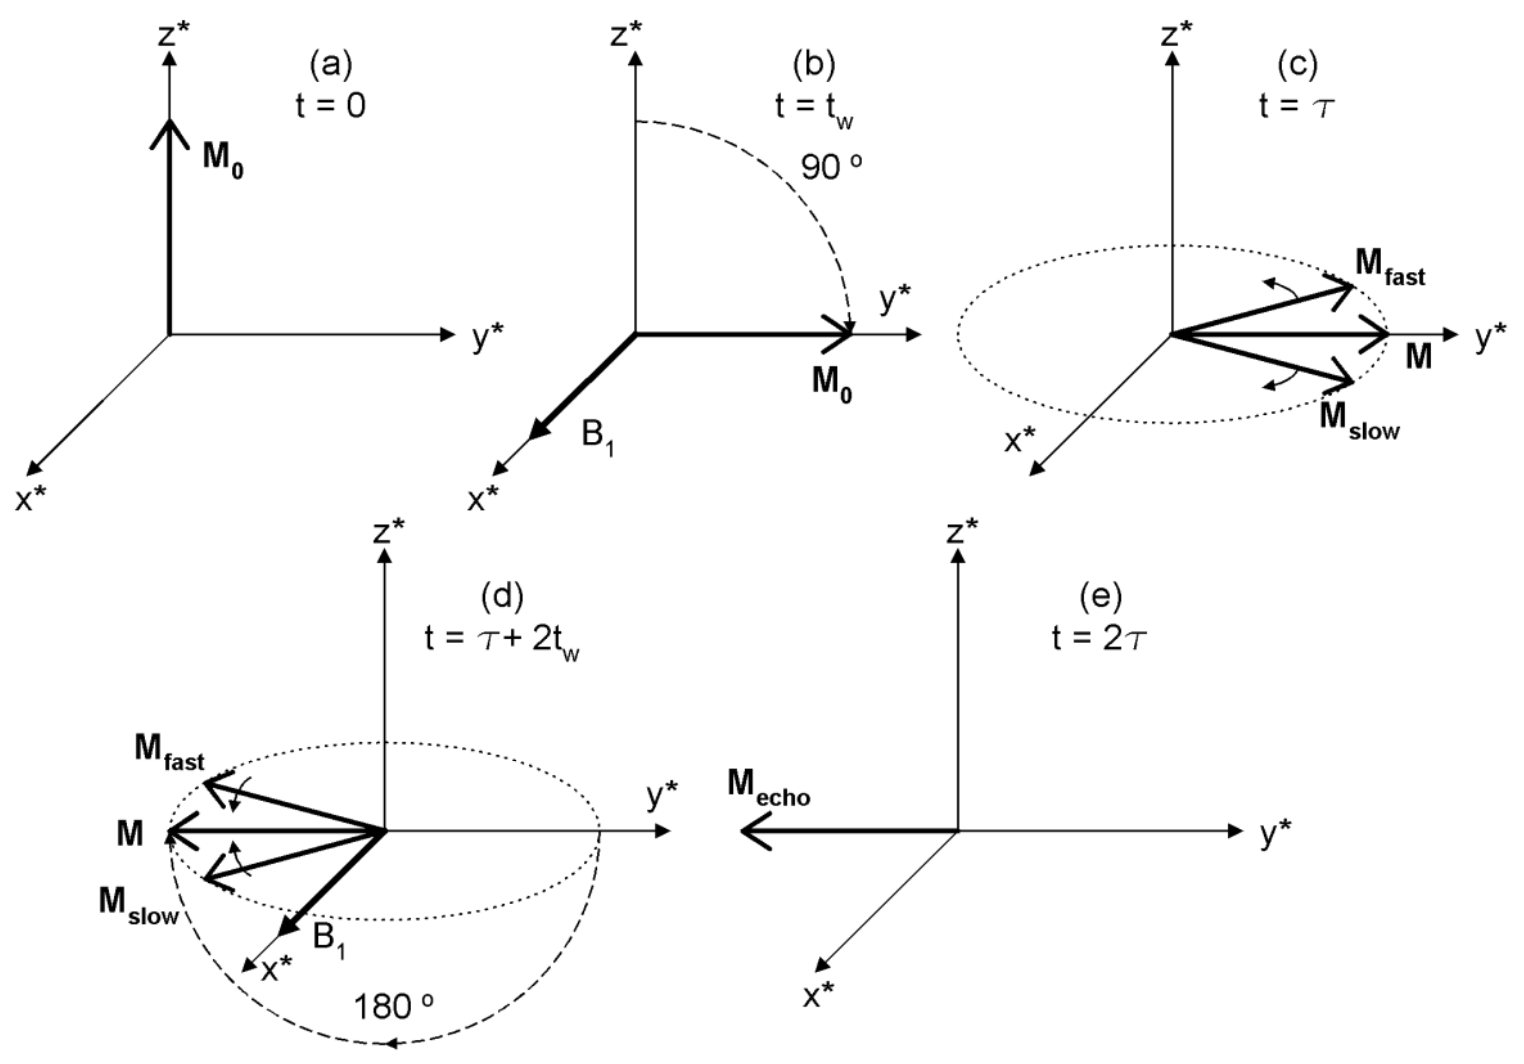
\includegraphics[width=0.5\linewidth]{figures/90-180-sequence.png}
    \end{figure}
    \begin{equation*}
        \lightning\quad\text{Echo amplitude} < \text{initial signal}
    \end{equation*}
    Loss of information must arise from time-dependent (stochastic) fluctuations
\end{frame}

%------------------------------------------------

\begin{frame}{Phase accumulation}
    Each spin accumulates a phase
    \begin{equation*}
        \phi (t) =\gamma \int_0^t \mathfrak{B} (t^\prime) dt^\prime
    \end{equation*}
    \begin{itemize}
        \item[$\bullet$] If $\mathfrak{B}$ is static, the phase evolution is deterministic
        \item[$\bullet$] If $\mathfrak{B}$(t) fluctuates, the phase becomes random
    \end{itemize}
    The signal is thus given by
    \begin{equation*}
        S(t)=\sum_{k=1}^N e^{i\phi_k (t)} \quad\Longrightarrow\quad S(t)=\left\langle e^{i\phi(t)}\right\rangle
    \end{equation*}
\end{frame}

%------------------------------------------------

\begin{frame}{Gaussianity of the stochastic field}
    Say $\mathfrak{B}(t) = \sum_i^N b_i (t)$, where the $b_i$ are
    \begin{itemize}
        \item zero-mean
        \item weakly correlated
        \item of the same order
    \end{itemize}
    Then for large $N$,
    \begin{equation*}
        \mathfrak{B}(t) \sim \mathcal{N}\left(0, \Delta^2 \right)
    \end{equation*}
    This is insufficient for a full characterization; indeed, we need
    \begin{equation*}
        C(T) = \left\langle \mathfrak{B}(t) \mathfrak{B}(t+T)\right\rangle
    \end{equation*}
    -- the autocorrelation function of the field
\end{frame}

%------------------------------------------------

\begin{frame}{Field correlations}
    $\phi (t)\sim\mathcal{N}\left(0,\left\langle \phi^2(t)\right\rangle\right)$ as a linear functional of a Gaussian process
    \begin{equation*}
        \left\langle e^{i\phi (t)}\right\rangle = e^{-\frac{1}{2}\left\langle \phi^2(t)\right\rangle}
    \end{equation*}
    Phase variance is determined entirely by the time correlations of the field:
    \begin{equation*}
        \left\langle\phi^2(t)\right\rangle = \gamma^2\int_0^t \int_0^t \left\langle \mathfrak{B}(t_1) \mathfrak{B}(t_2)\right\rangle\,dt_1dt_2
    \end{equation*}
    What correlation structure of $\mathfrak{B}(t)$ produces 
    \begin{equation*}
        \left\langle \phi^2(t)\right\rangle \propto t \quad\Longrightarrow\quad M_{xy}(t)\sim e^{-t}?
    \end{equation*}
\end{frame}

%------------------------------------------------

\begin{frame}{Modeling the fluctuating field}
    \begin{block}{Ornstein-Uhlenbeck process}
        Describes a field that randomly fluctuates with amplitude $\sigma$, but relaxes back to zero over a timescale $\tau_c$
        \begin{equation*}
            d\mathfrak{B}_t = -\frac{1}{\tau_c}\mathfrak{B}_tdt + \sigma dW_t 
        \end{equation*}
        \begin{itemize}
            \item[$\bullet$] $dW_t \sim \mathcal{N}(0,dt)$ -- Gaussian white noise
        \end{itemize}
    \end{block}
    \textbf{Correlation function}
    \begin{equation*}
       C(T)=\left\langle \mathfrak{B}(t) \mathfrak{B}(t+T)\right\rangle = \Delta^2 e^{-\left\lvert T \right\rvert /\tau_c}
    \end{equation*}
    \textbf{Phase variance}
    \begin{equation*}
        \left\langle \phi^2(t)\right\rangle \sim 
        \begin{cases}
            t^2,&\quad t\ll \tau_c\\
            t,&\quad t\gg\tau_c
        \end{cases}
        \quad\Longrightarrow\quad \boxed{M_{xy} (t) \sim e^{-t},\quad t\gg\tau_c}
    \end{equation*}
\end{frame}

%------------------------------------------------

\begin{frame}{Simulating the OU process}
    Under an isotropicity assumption, there is a mapping $\left(T_1,T_2\right) \mapsto \left(\tau_c, \Delta^2\right)$:
    \begin{equation*}
        \underbrace{\tau_c = \frac{1}{\omega_0}\sqrt{2\left(\frac{T_1}{T_2}-1\right)}}_{\text{memory time of fluctuations}},\qquad \underbrace{\Delta^2 = \frac{1}{4\gamma^2 T_1 \tau_c}\left( 1+\omega_0^2\tau_c^2\right)}_{\text{fluctuation amplitude}}
    \end{equation*}
    We can feed these parameters into
    \begin{equation*}
        \phi_{\text{echo}}(2\tau) = \gamma\left(\int_0^{\tau}\mathfrak{B}_z(t)\,dt^\prime - \int_\tau^{2\tau}\mathfrak{B}_z(t)\,dt^\prime\right)
    \end{equation*}
    and predict the echo amplitude via
    \begin{equation*}
        S(2\tau) \propto \left\lvert\left\langle e^{i\phi(2\tau)}\right\rangle\right\rvert
    \end{equation*}
\end{frame}

%------------------------------------------------

\begin{frame}{Experimental objectives}
    \begin{alertblock}{\textbf{Goal}}
        Test whether OU-derived parameters from $T_1,T_2$ predict spin echo decay
        \begin{itemize}
            \item[$\bullet$] Extract $\tau_c,\Delta^2$ from $T_1,T_2$
            \item[$\bullet$] Predict echo amplitude
            \item[$\bullet$] \hl{Compare with experiment}
        \end{itemize}
    \end{alertblock}
    Samples probe different correlation-time regimes
    \begin{table}[h]
        \centering
        \begin{tabular}{lccc}
            \hline
            \textbf{Sample} & \textbf{Dynamics} & $\boldsymbol{\tau_c}$ \textbf{Regime} & \textbf{Purpose} \\
            \hline
            Light Mineral Oil 
            & Fast 
            & $\tau_c \ll 1/\omega_0$ 
            & Validation \\

            Heavy Mineral Oil 
            & Intermediate
            & $\tau_c \sim 1/\omega_0$ 
            & Tests limits \\

            Vaseline (optional) 
            & Slow
            & $\tau_c \gg 1/\omega_0$ 
            & Failure case \\
            \hline
        \end{tabular}
    \end{table}
\end{frame}

%------------------------------------------------

\begin{frame}{Magnetization dynamics ($T_1$)}
    Longitudinal magnetization relaxes exponentially to equilibrium. Assuming $M(0) = 0$,
    \begin{equation*}
        M_z(t) = M_0 (1-e^{-t/T_1})
    \end{equation*}

    \begin{minipage}[t]{0.5\textwidth}
        \begin{figure}
            \centering
            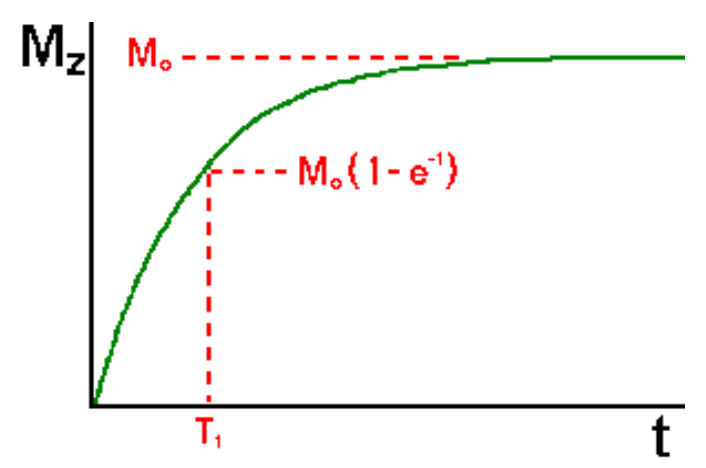
\includegraphics[width=0.65\linewidth]{figures/T1_theory.png}
            \captionof{figure}{Magnetization vs. time for a sample placed in a magnetic field [TeachSpin Pulsed/CW NMR Manual]}
        \end{figure}
    \end{minipage}
    \hfill
    \begin{minipage}[t]{0.45\textwidth}
        \begin{block}{$T_1$ -- Spin-lattice relaxation time}
            Characteristic timescale of relaxation toward thermal equilibrium, caused by exchange of
            \begin{itemize}
                \item \textbf{energy}
                \item \textbf{angular momentum}
            \end{itemize}
            \textit{from} nuclei \textit{to} lattice
        \end{block}
    \end{minipage}
\end{frame}

%------------------------------------------------

\begin{frame}{Measuring $T_1$: inversion recovery}
    \begin{minipage}[t]{0.5\textwidth}
        \begin{figure}
            \centering
            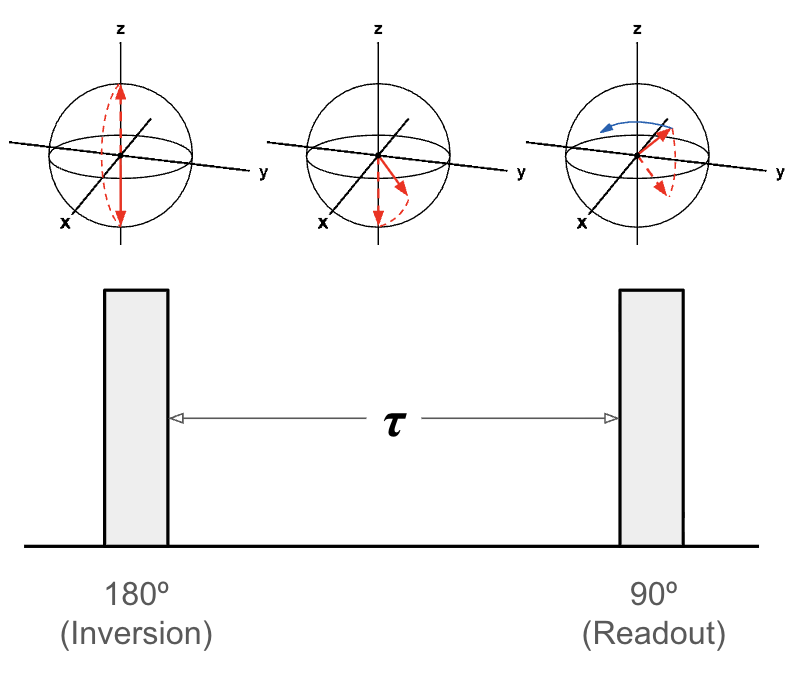
\includegraphics[width=\linewidth]{figures/inv-recovery.png}
        \end{figure}
    \end{minipage}
    \hfill
    \begin{minipage}[t]{0.48\textwidth}
        \begin{figure}
            \centering
            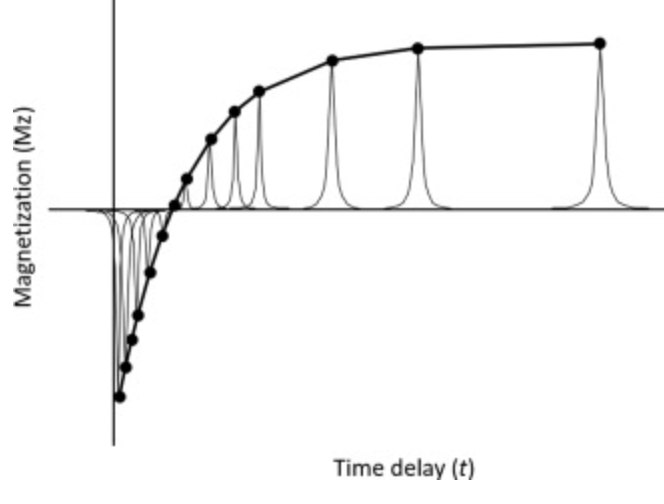
\includegraphics[width=0.8\linewidth]{figures/inv-rec-curve.png}
            \caption{[ScienceDirect -- Inversion Recovery]}
        \end{figure}
        \begin{equation*}
            M_z (t) = M_0(1-2e^{-t/T_1})
        \end{equation*}
    \end{minipage}
\end{frame}

%------------------------------------------------

\begin{frame}{$T_1$ measurements}
    Env. Out gives only $S(\tau) \propto \left\lvert M_z (\tau)\right\rvert$, so we adjust the fit:
    \begin{equation*}
        S(\tau) = A\left\lvert 1-2e^{-\tau/T_1} \right\rvert + C
    \end{equation*}\\[-0.5em]
    \begin{minipage}[t]{0.49\textwidth}
        \begin{equation*}
            T_{1,\text{light}}=528 \pm 1\,\mathrm{ms}
        \end{equation*}
        \vspace{-20pt}
        \begin{figure}
            \centering
            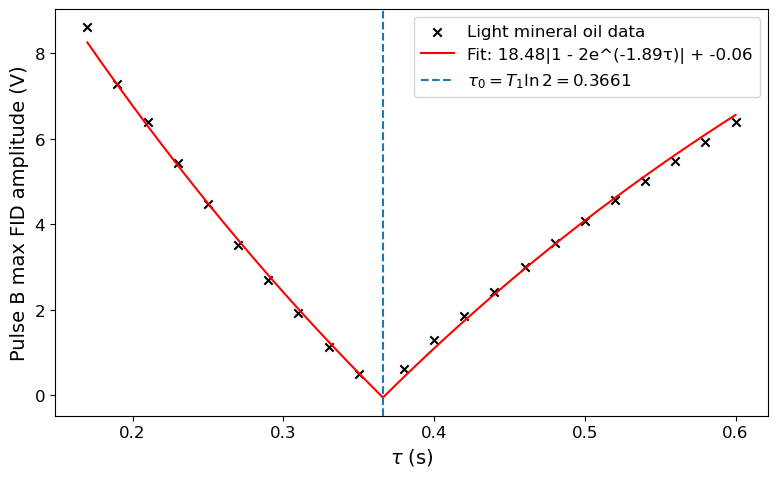
\includegraphics[width=\linewidth]{figures/light_oil_T1.png}
        \end{figure}
    \end{minipage}
    \hfill
    \begin{minipage}[t]{0.49\textwidth}
        \begin{equation*}
            T_{1,\text{heavy}}=31.8\pm 0.1\,\mathrm{ms}
        \end{equation*}
        \vspace{-20pt}
        \begin{figure}
            \centering
            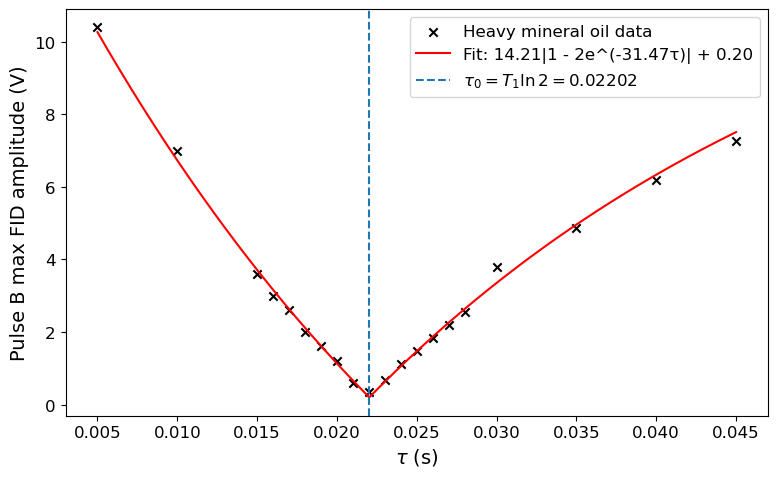
\includegraphics[width=\linewidth]{figures/heavy_oil_T1.png}
        \end{figure}
    \end{minipage}
\end{frame}

%------------------------------------------------

\begin{frame}{Measuring $T_2$: spin echo decay}
    \begin{figure}
        \centering
        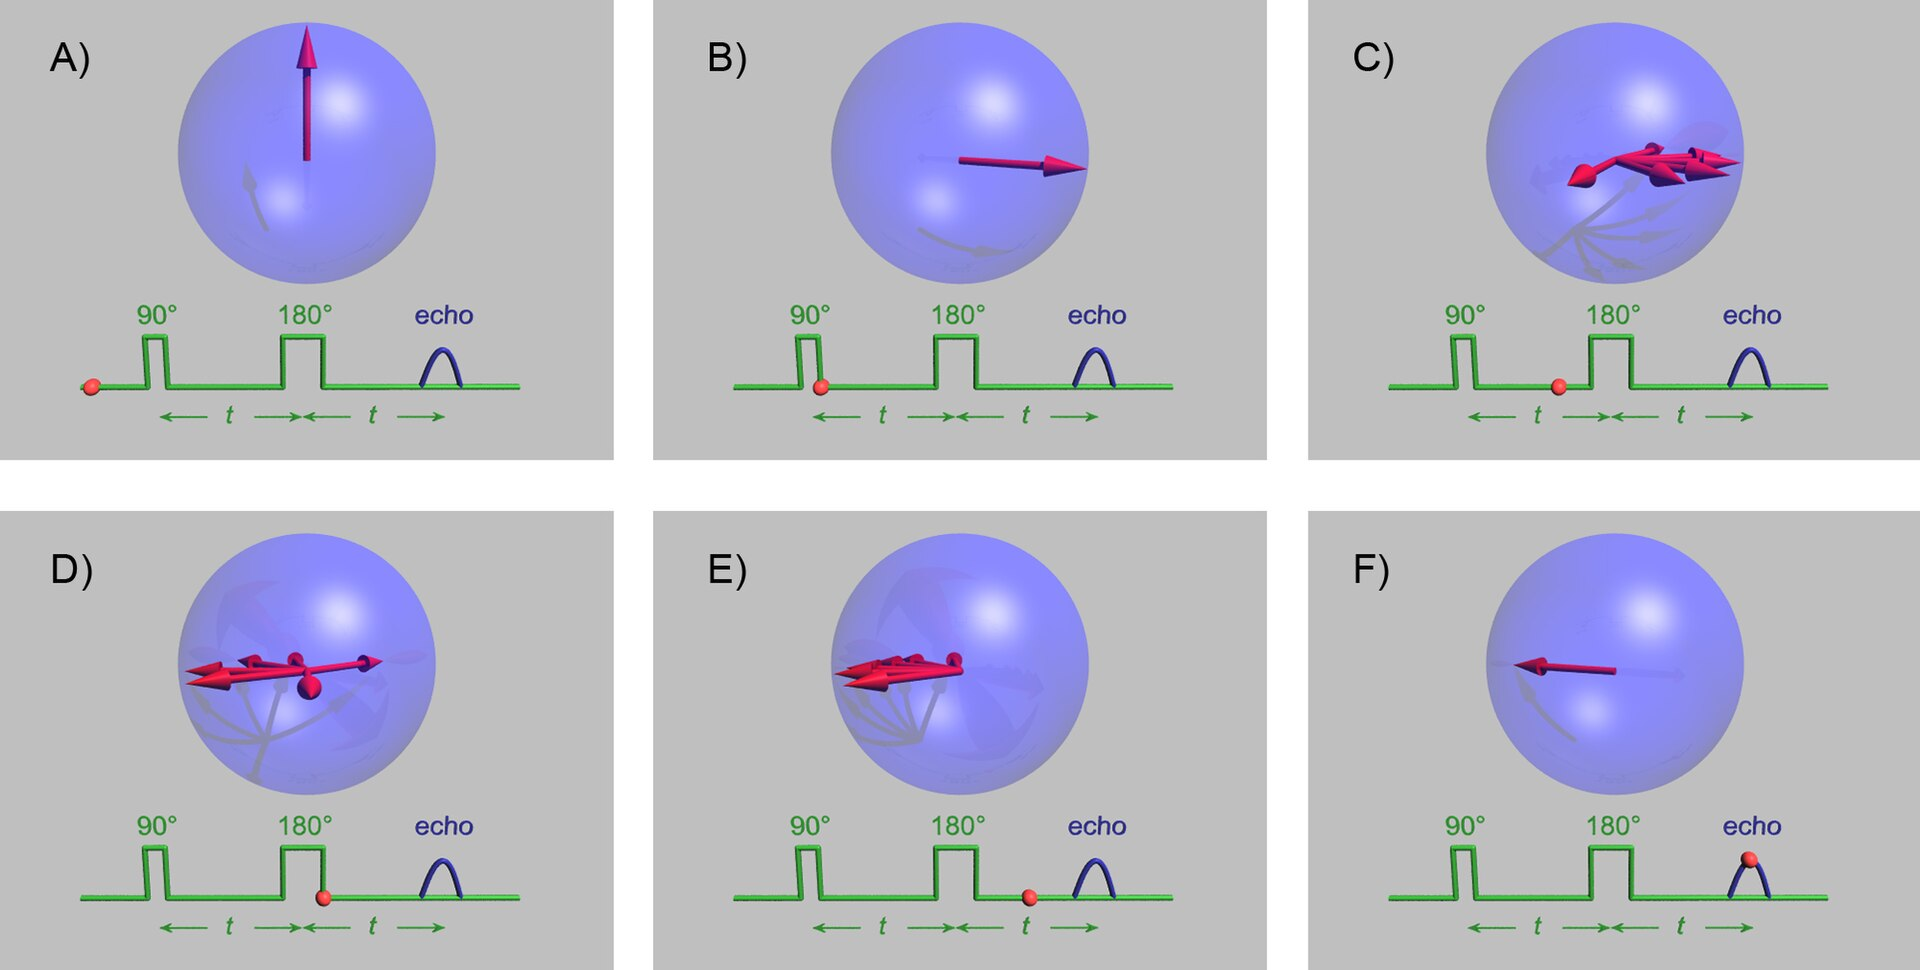
\includegraphics[width=0.75\textwidth]{figures/SpinEcho_GWM_stills.jpg}
    \end{figure}
    \begin{equation*}
        M_{xy}(2\tau) = M_0 e^{-2\tau/T_2}\quad\Longrightarrow\quad S(2\tau)=Ae^{-2\tau/T_2}+C
    \end{equation*}
\end{frame}

%------------------------------------------------

\begin{frame}{$T_2$ measurements}
    \begin{minipage}[t]{0.49\textwidth}
        \begin{equation*}
            T_{2,\text{light}}=39.3\pm 0.5 \,\mathrm{ms}
        \end{equation*}
        \vspace{-20pt}
        \begin{figure}
            \centering
            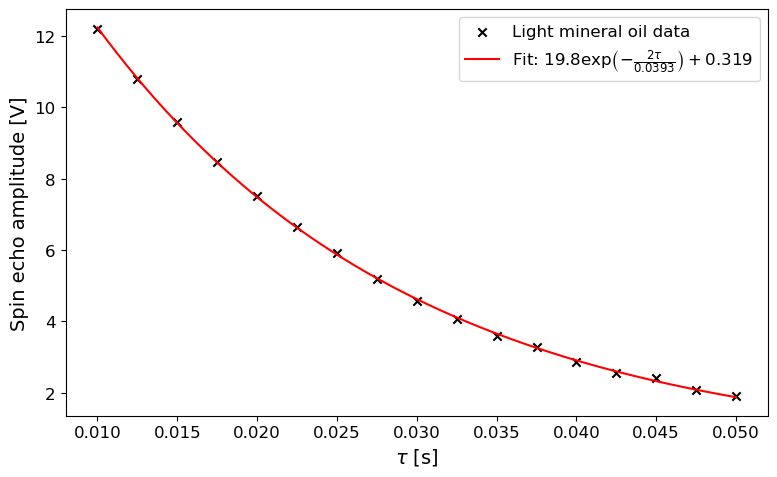
\includegraphics[width=\linewidth]{figures/light_oil_T2.png}
        \end{figure}
    \end{minipage}
    \hfill
    \begin{minipage}[t]{0.49\textwidth}
        \begin{equation*}
            T_{2,\text{heavy}}=20.2\pm 0.5\,\mathrm{ms}
        \end{equation*}
        \vspace{-20pt}
        \begin{figure}
            \centering
            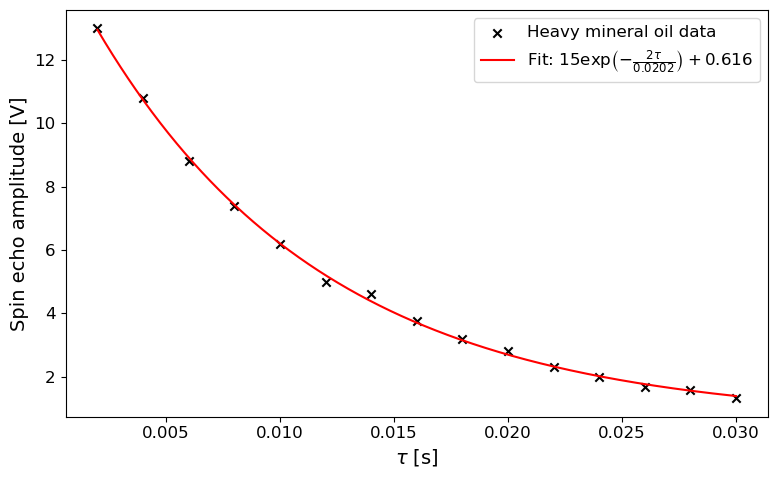
\includegraphics[width=\linewidth]{figures/heavy_oil_T2.png}
        \end{figure}
    \end{minipage}
\end{frame}

%------------------------------------------------

\begin{frame}{Simulation parameters}
    \begin{table}[h]
    \centering

    \begin{tabular}{lccc}
        \hline
        Sample & $T_1$ (ms) & $T_2$ (ms) & $f_{\mathrm{rec}}$ (MHz) \\
        \hline
        Light Oil & 528 & 39.3 & 21.12730 \\
        Heavy Oil & 31.8 & 20.2 & 21.02330 \\
        \hline
    \end{tabular}

    \vspace{0.5em}

    $\Downarrow$

    \vspace{0.5em}

    \begin{tabular}{lccc}
        \hline
        Sample & $\tau_c$ (ns) & $\Delta^2\,(\mathrm{G}^2)$ & $\sigma\,(\mathrm{T}\cdot\mathrm{s}^{-1/2})$ \\
        \hline
        Light Oil & {\color{red} 37.6} & 0.45 & 0.49 \\
        Heavy Oil & 8.09 & 2.91 & 2.68 \\
        \hline
    \end{tabular}

    \caption{Extraction of OU parameters from measured relaxation times.}
    \end{table}
\end{frame}

%------------------------------------------------

\begin{frame}{Simulated OU field and autocorrelation}
    \begin{figure}
        \centering
        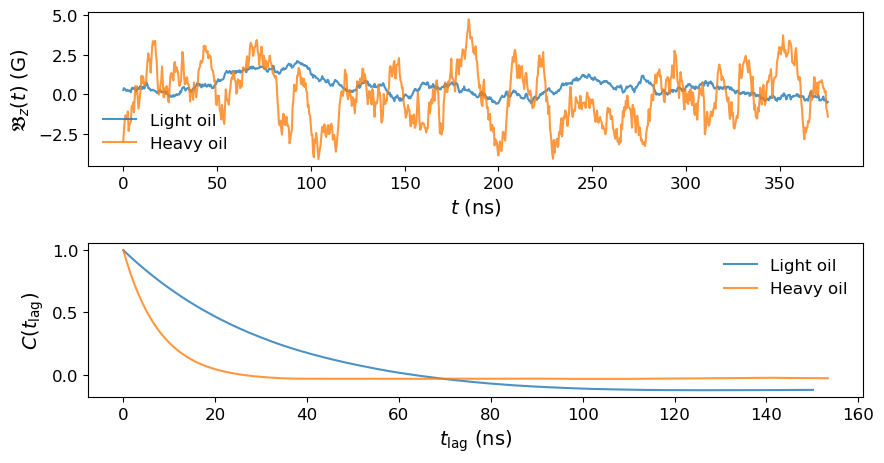
\includegraphics[width=0.78\linewidth]{figures/OU_field_autocorr.png}
        \caption{OU field $\mathfrak{B}_z(t)$ realization and autocorrelation $C(t_{\text{lag}})$ over 2000 realizations}
    \end{figure}
\end{frame}

%------------------------------------------------

\begin{frame}{Simulated phase accumulation}
    For illustration purposes, we pick $\tau = \tau_{c,\text{light}}$, and $\lvert S(2\tau) \rvert = \left\lvert\left\langle \exp{i \phi(2\tau)} \right\rangle \right\rvert$
    \begin{figure}
        \centering
        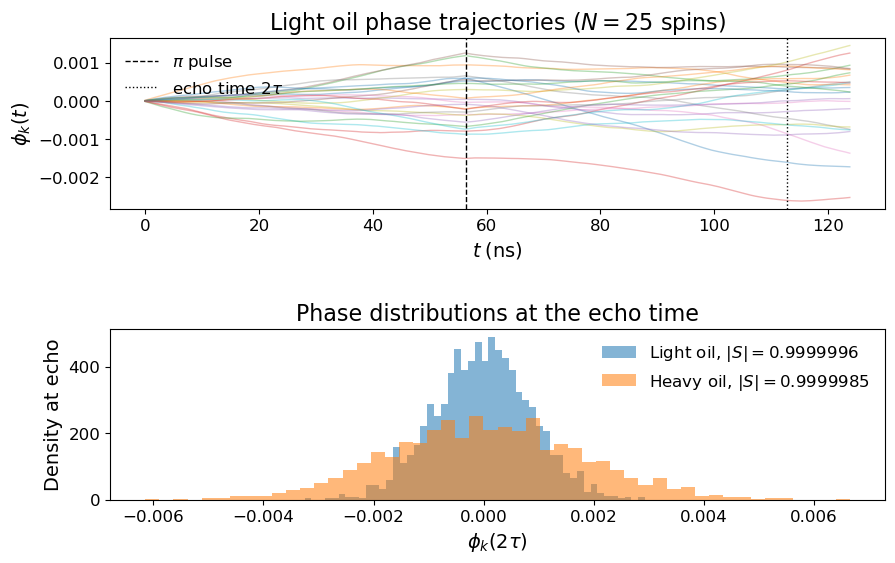
\includegraphics[width=0.68\linewidth]{figures/phase_distribution.png}
    \end{figure}
\end{frame}

%------------------------------------------------

\begin{frame}{Experimental v.s. simulated echo decay}
    \begin{minipage}[t]{0.53\textwidth}
        \begin{figure}
            \centering
            
\includegraphics[width=\linewidth]{figures/OU_vs_exp.png}
        \end{figure}
    \end{minipage}
    \hfill
    \begin{minipage}[t]{0.46\textwidth}
        Potential failure modes:
        \begin{itemize}
            \item[$\bullet$] Account for the effect of $\mathfrak{B}_{xy}$ (energy relaxation),
            \item[$\bullet$] Real liquids have multiple motional process
            \begin{equation*}
                C(t) = \sum_i \Delta_i^2 \exp{(-\lvert t \rvert/\tau_i)},
            \end{equation*}
            \item[$\bullet$] Molecular diffusion through gradients
            \begin{equation*}
                S(2\tau) \sim \exp{(-D\gamma G^2 \tau^3)},
            \end{equation*}
            \item[$\bullet$] Circular validation: test on a different dataset.
        \end{itemize}
    \end{minipage}
\end{frame}

%------------------------------------------------

\begin{frame}{Conclusion}
    \textbf{Key result}
    \begin{itemize}
        \item The OU model \textit{qualitatively} predicts spin echo decay, but systematically underestimates relaxation.
    \end{itemize}
    \textbf{Regime dependence}
    \begin{itemize}
        \item Heavy oil: strong deviation
        \item Light oil: better agreement
    \end{itemize}
    \textbf{Interpretation}
    \begin{itemize}
        \item Extend model: multi-timescale correlations or include transverse fluctuations
    \end{itemize}
\end{frame}

\end{document}